\chapter{Approach}
\label{chap:approach}
% ================================================================
% DATA DESCRIPTION
\section{Data Description}
In this project, BCI2000, Competition III, Dataset II was used, due to being accurate, free, provides 64 channels and quite a number of papers was based on it which provides a good reference for comparison of classifiers and the corresponding accuracy. In addition to the competition's dataset, we recorded our own dataset from 2 subjects. In total, the competition's dataset has 2 subjects A and B, the recorded dataset has another 2 subjects C and D.\par
% ----------------------------------------------------------------
\subsection{Paradigm}
The \ac{p300} speller in the competition was like the following; the user is shown a 6x6 matrix of characters (Figure \ref{fig:p300-speller}). Each row and column is intensified in a random sequence. Then, the user focuses his gaze on one of the 36 cells of the matrix. The sequence of 12 intensifications (6 rows + 6 columns) which results in an oddball paradigm where the intensification of the focused character represents the infrequent event and the other intensifications + no intensifications represents the frequent event. The event which is infrequent will result in a \ac{p300} response, while the frequent event will have no change on the signal (Figure \ref{fig:p300-signal}). \cite{article1}\par
\begin{figure}
    \centering
    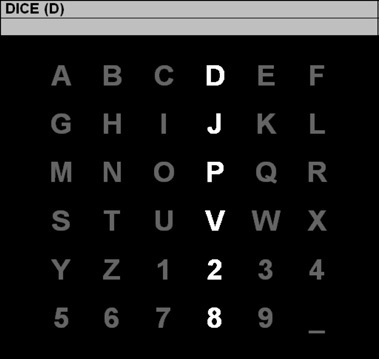
\includegraphics[width=\figureWidth]{images/approach/p300_speller.jpg}
    \caption{\ac{p300} Speller: Representation of the intensification of the 4th column \cite{article1}.}
    \label{fig:p300-speller}
\end{figure}
% ----------------------------------------------------------------
\subsection{Recording}
\subsubsection{Competition's Data}
In the competition's dataset (Subjects A and B), signals are filtered from 0.1 – 60Hz and digitized at 240Hz (Each 240 samples corresponds to 1 second). The 12 sets of intensifications were repeated 15 times for each character resulting in 180 total intensifications per epoch (character) into 64 channels EEG (Figure \ref{fig:competition-64-channels}). There are 185 epoch in total; 85 train and 100 test per subject.\par
\begin{figure}[!ht]
    \centering
    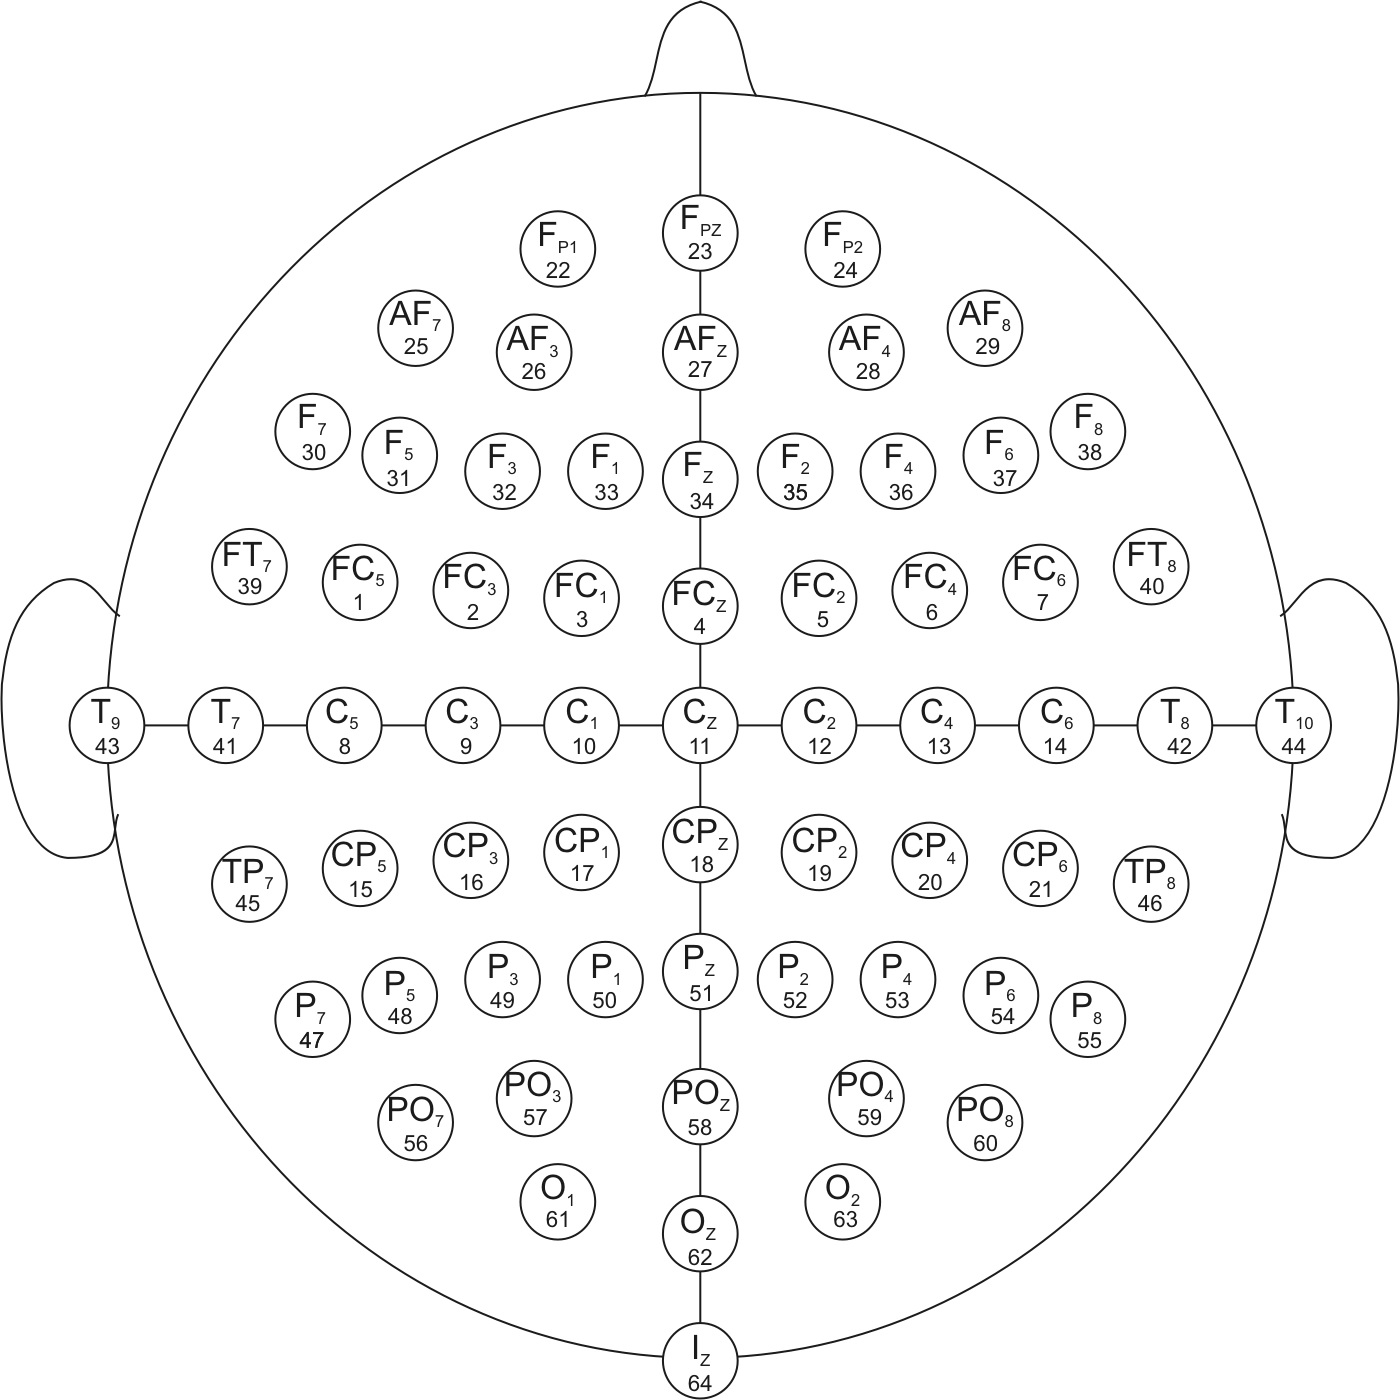
\includegraphics[width=\figureWidth]{images/approach/competition_64_channels.jpg}
    \caption{Mapping of sesnors on the scalp according to the competition's dataset description.}
    \label{fig:competition-64-channels}
\end{figure}
% ----------------------------------------------------------------
\subsubsection{Recorded Data}
In the dataset we recorded (Subjects C and D), signals are digitized at 128Hz (Each 128 samples corresponds to 1 second). The 12 sets of intensifications were repeated 15 times for each character resulting in 180 total intensifications per epoch into 14 channels EEG (Figure \ref{fig:emotiv-14-channels}, (a)). There are 72 epoch in total; 57 train and 15 test per subject.\par.
\begin{figure}
    \centering
    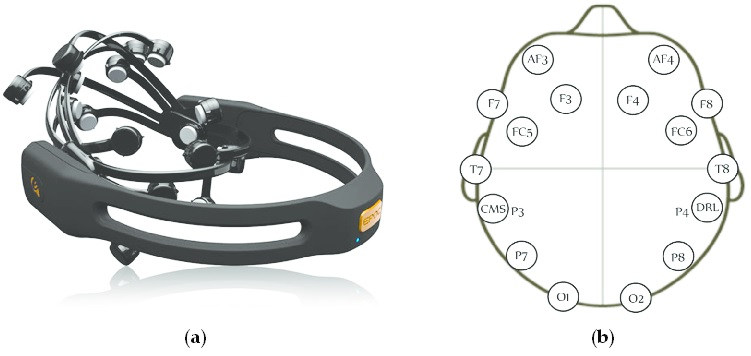
\includegraphics[width=\figureWidth]{images/approach/emotiv_14_channels.jpg}
    \caption{Mapping of sesnors on the scalp in EMOTIV EPOC+ headset \cite{article8}.}
    \label{fig:emotiv-14-channels}
\end{figure}
% ----------------------------------------------------------------
Note that, only 14 channels were recorded for subjects (C, D) due to hardware limitation (EMOTIV EPOC+). The 14 channels are AF3, F7, F3, P3, T7, P7, O1, O2, P8, T8, P4, F4, F8 and AF4 (Figure \ref{fig:emotiv-14-channels}, (b))\par
% ----------------------------------------------------------------
\subsection{Data Explanation}
\label{subsection:data-explanation}
The competition's dataset has 5 arrays descried below (the description provided by the competition for dataset 2).
\begin{tabbing}
    Title:\quad \quad \quad \quad \quad \=Description\kill
    Signal:         \>signal of each channel (Figure 2.5)\\
                    \>Type: 3D Array\\
                    \>Shape (Dimension): (85, 7794, 64)\\
    \newline\\
    TargetChar:     \>The chosen character for each epoch\\
                    \>Type: String\\
                    \>Length: 85\\
    \newline\\
    Flashing:	    \>0	when NO row/column is intensified\\
                    \>1	when row/column is intensified\\
                    \>Type: 2D Array\\
                    \>Shape (Dimension): (85, 7794)\\
    \newline\\
    StimulusCode:	\>0	when NO row/column is intensified\\
                    \>1 ... 6	when intensified column (1 is left-most column)\\
                    \>7 ... 12	when intensified row (1 is upper-most row)\\
                    \>Type: 2D Array\\
                    \>Shape (Dimension): (85, 7794)\\
                    \>Figure \ref{fig:row-column-numbering}\\
    \newline\\
    StimulusType:	\>0	when NO row/column is intensified\\
    		        \>1	when row/column contains the chosen character\\
                    \>Type: 2D Array\\
                    \>Shape (Dimension): (85, 7794)\\
\end{tabbing}\par
\begin{figure}
    \centering
    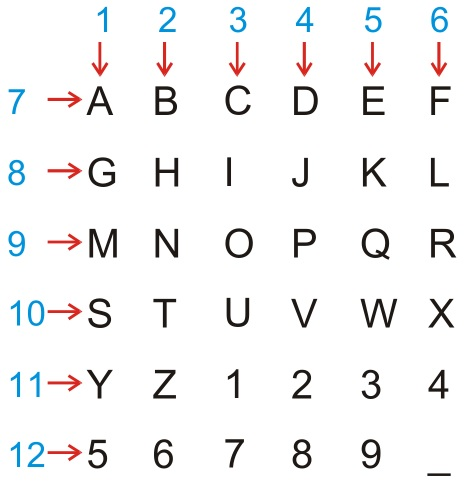
\includegraphics[width=\figureWidth]{images/approach/row_column_numbering.jpg}
    \caption{Row/Column numbering values.}
    \label{fig:row-column-numbering}
\end{figure}
% ----------------------------------------------------------------
Note: This is dimension of the train dataset. If dimension of the test dataset is needed, substitute 85 with 100.\par
% ----------------------------------------------------------------
Note: TargetChar, StimulusType are only provided for training dataset.\par
% ----------------------------------------------------------------
Note: Since algorithm has been updated, only Signal, TargetChar, StimulusCode and the matrix used for training are needed to train the \ac{ml} model.\par
% ----------------------------------------------------------------
\clearpage
% ================================================================






% DATA PRE-PROCESSING
\section{Data Pre-processing}
% ----------------------------------------------------------------
\subsection{Average of Repetitions}
Average of the all repetitions for both the competition's dataset and the recorded dataset were done according to the proposed algorithm provided by the competition in the example file. A modified version is that, we search for 2 consecutive samples in StimulusCode current and previous. If the current sample is zero, and the previous sample is non-zero, then that means there was a transition from intensification to no intensification. Then we sum the samples of the window needed (i.e. 192 samples = 800ms for competition's dataset) to the corresponding previous intensification samples.\par
% ----------------------------------------------------------------
For example, in the competition's dataset, according to Sub-Section \ref{subsection:data-explanation}, the train set has dimension (85, 7794, 64), after calculating the average the repetitions the new dimensions will be (85, 12, 192, 64).\par
% ----------------------------------------------------------------
Note: 7794 and 192 because the digitization rate for the the used headset in the competition is 240 Hz.\par
% ----------------------------------------------------------------
In the recorded dataset, the train set has dimension (57, 4600, 14), after calculating the average the repetitions the new dimensions will be (57, 12, 102, 14).\par
% ----------------------------------------------------------------
Note: 4600 and 102 because the digitization rate for the EMOTIV headset is 128 Hz.\par
% ----------------------------------------------------------------
\subsection{Filters}
\subsubsection{Common Average Reference (CAR)}
The signals were filtered using \ac{car} filter (Equation \ref{eq:car}). By subtracting the mean of samples across all channels at certain time from signals at the same certain time helps to remove the noise in some channels.\par
\begin{equation}
    f_c(t) = s_c(t) - \frac{1}{N} \sum_{i=1}^N s_i(t)
    \label{eq:car}
\end{equation}
% ----------------------------------------------------------------
$f_c(t)$ is the filtered signal for electrode (channel) c at time t. $s_c(t)$ is the raw signal for electrode (channel) c at time t. $\frac{1}{N} \sum_{i=1}^{N} s_i(t)$ is the mean of channels at time t.\par
% ----------------------------------------------------------------
\subsubsection{Moving Average}
After that, Moving average filter was applied in order to remove noise within time units per channel (Equation \ref{eq:ma}).\par
\begin{equation}
    f_c(t) =  \frac{1}{M} \sum_{i=t}^{t+M} s_c(i)
    \label{eq:ma}
\end{equation}
% ----------------------------------------------------------------
$f_c(t)$ is the filtered signal for electrode (channel) c at time t. $\frac{1}{M} \sum_{i=t}^{t+M} s_c(i)$ is the mean consecutive M signal where M is the moving average filter value.\par
% ----------------------------------------------------------------
In the competition's dataset, it will be set to 25 \cite{inproceedings1}. However, in the recorded dataset, it will be set to 13 \cite{inproceedings2}.\par
% ----------------------------------------------------------------
\subsubsection{Z-Score}
After applying moving average, the signals were scaled using Z-Score (Equation \ref{eq:zs}).\par
\begin{equation}
    f_{cj} =  \frac{s_c(j) - \mu_c}{\sigma_c}
    \label{eq:zs}
\end{equation}
% ----------------------------------------------------------------
$f_{cj}$ is the filtered signal for electrode (channel) c and feature j. $s_c(j)$ is the signals for electrode c and feature j. $\mu_c$ is the mean of signals recorded on electrode c. $\sigma_c$ is the standard deviation of signals recorded on electrode c.\par
% ----------------------------------------------------------------
\subsubsection{Decimation}
Finally, the filtered signal is decimated by certain value. Assume decimation value of n. This means we will take 1 signal as a feature every n signals.\par
% ----------------------------------------------------------------
In the competition's dataset, it will be set to 12 \cite{inproceedings1}. However, in the recorded dataset, it will be set to 6 \cite{inproceedings2}.\par
% ----------------------------------------------------------------
\clearpage
% ================================================================





% FEATURE EXTRACTION
\section{Feature Extraction}
\subsection{Channel Selection}
\label{subsection:channel-selection}
Data segments of extracted data can vary a lot since the elicited signal appears from 250 - 500ms. Most papers \cite{inproceedings1, inproceedings2, article1, article2} uses data segments that vary from 600 - 1000ms. However, in this project, 0 - 800ms data segment is going to be used.\par
% ----------------------------------------------------------------
In the competition's dataset, the number of samples will be 192 sample. There are 2 sets of channels are going to be used; the first will consist of 8 channels (Fz, Cz, Pz, P3, P4, PO7, PO8 and
Oz) (Figure \ref{fig:competition-8-channels}) \cite{inproceedings1, article1}. And the other set will consist of all the 64 channels.\par
\begin{figure}
    \centering
    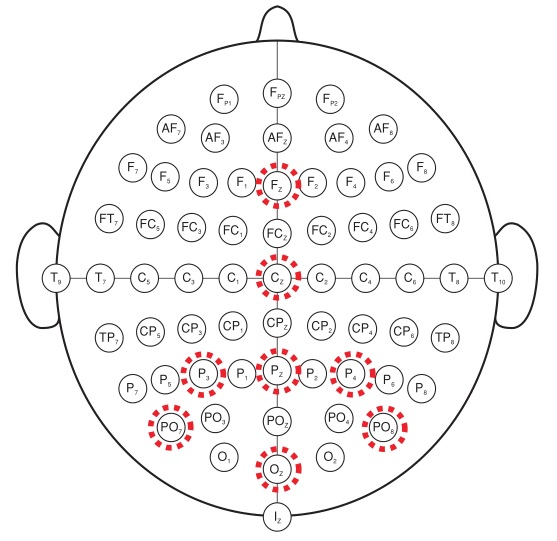
\includegraphics[width=\figureWidth]{images/approach/competition_8_channels.jpg}
    \caption{Most effective electrodes according to Dean and Sellers \cite{article1}.}
    \label{fig:competition-8-channels}
\end{figure}
% ----------------------------------------------------------------
On the other hand, then number of sample for the recorded dataset will be 102 sample. And all the 14 channels are going to be used (Figure \ref{fig:emotiv-14-channels}).
% ----------------------------------------------------------------
\subsection{Feature Vector Concatenation}
After channel selection, all the extracted channels will then be concatenated and passed to the classifier. This approach was used to allow the use of more than 1 channel to determine the \ac{p300}.\par
% ----------------------------------------------------------------
\clearpage
% ================================================================



% CLASSIFICATION
\section{Classification}
Since \ac{p300} is an oddball paradigm, meaning that it is either frequent or infrequent event. The whole classification problem is a binary one. It is either \ac{p300} or Non-\ac{p300}. In this project, linear classifiers whose decision boundary will be like Equation \ref{eq:linear-classifier-boundary}.\par
\begin{equation}
    w^T x + b = 0
    \label{eq:linear-classifier-boundary}
\end{equation}
% ----------------------------------------------------------------
$w$ is the weight (line slope). $x$ is the feature vector (sample). $b$ is the bias term (line shift).\par
% ----------------------------------------------------------------
\subsection{Class Construction and Character Prediction}
Since the problem is a binary classification problem, we will set the the target class to be 1 for the intensification with \ac{p300}, and -1 (or 0) for the intensification with Non-\ac{p300}.\par
Since the \ac{p300} Speller is only has 2 \ac{p300} events (1 for each dimension row/column), the character prediction will be based on the maximum value from the score function (decision function).\par
% ----------------------------------------------------------------
Note that, the higher the score (score is the predicted y label) (Equation \ref{eq:score}), the further away from the corresponding line on the hyper plane, which makes it more accurate for a \ac{p300} elicit (Equation \ref{eq:predicted-row}, and Equation \ref{eq:predicted-column}) \cite{inproceedings1, inproceedings2, article1}.\par
\begin{equation}
    score = w^T x
    \label{eq:score}
\end{equation}
\begin{equation}
    row = max(w^T x_{7..12})
    \label{eq:predicted-row}
\end{equation}
\begin{equation}
    column = max(w^T x_{1..6})
    \label{eq:predicted-column}
\end{equation}
% ----------------------------------------------------------------
$w$ is the weight. $x$ is the feature vector. $max(..)$ is a function to get max of given values. Check Sub-Section \ref{subsection:data-explanation} for row/column numbering values.\par
% ----------------------------------------------------------------
\subsection{Linear Discriminant Analysis (LDA)}
\ac{lda} is the most basic linear classifier which is based on least squared error. The weight vector is calculated based on Equation \ref{eq:lda-weight-calculation} \cite{inproceedings1}.\par
\begin{equation}
    w = (X^T X)^{-1} X^T y
    \label{eq:lda-weight-calculation}
\end{equation}
% ----------------------------------------------------------------
$w$ is the weight. $X$ is the matrix with feature vectors as rows. $y$ is the vector that has the labels of each row within $X$.\par
% ----------------------------------------------------------------
For Example, in the competition's dataset, $X$ has dimension (1020, 128), and $y$ has dimension (1020). Note that, we are using 85 character (train dataset), 12 intensifications, 192 sample (0 - 800ms) and 8 concatenated channel.\par
\[85 \times 12 = 1020\]
\[\frac{192}{12} \times 8 = 128\]
% ================================================================


% Graphical User Interface (GUI)
\section{Graphical User Interface (GUI)}
The language used to make the \ac{gui} is python programming language. As for the \ac{gui} package itself (classes and functions) is called Tkinter.\par
% ----------------------------------------------------------------
The user is shown the matrix in Figure \ref{subfig:recorded-gui-non-intensification} for 2.5 seconds. Then, the intensifications of rows and columns starts (12 intensifications, 15 repetitions) as in Figure \ref{subfig:recorded-gui-intensification}, after that, the \ac{gui} halts for 2 seconds because the \ac{p300} takes time to take effect (300ms after the stimulus).\par
% ----------------------------------------------------------------
Note that, number 5 is highlighted in Figure \ref{subfig:recorded-gui-non-intensification} to signify that the user should focus on it in order to train it.\par
\begin{figure}[!ht]
    \centering
    \subfloat[
        Non-intensification state of the \ac{gui} (frequent event).
        \label{subfig:recorded-gui-non-intensification}
        ]{
            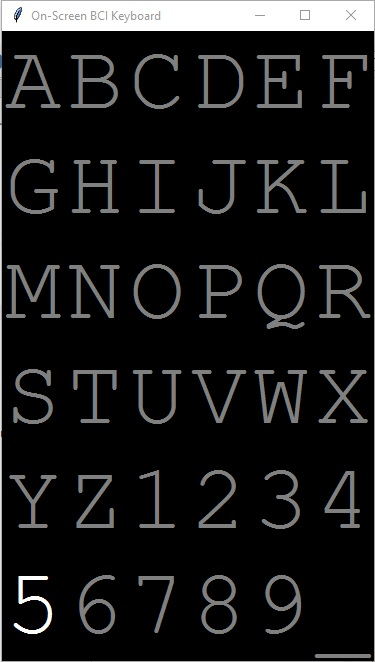
\includegraphics[width=\subFigureWidth]{images/approach/recorded_gui_non_intensification.jpg}
        }
    \hfill
    \subfloat[
        Intensification state of column 4 state of the \ac{gui} (infrequent event).
        \label{subfig:recorded-gui-intensification}
        ]{
            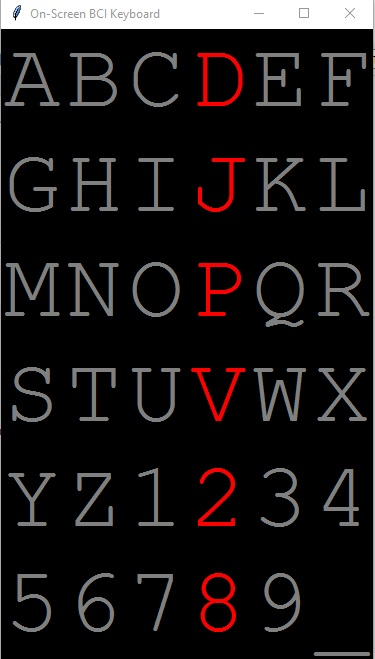
\includegraphics[width=\subFigureWidth]{images/approach/recorded_gui_intensification.jpg}
        }
    \caption{\ac{gui} used to record the dataset.}
    \label{fig:recorded-gui}
\end{figure}
% ----------------------------------------------------------------
\clearpage
% ================================================================
